Según se nos pide realizamos tres experimentos. En el primero encontramos el mejor tamaño de cuadrícula
teniendo como criterio de ordenación el tiempo que tarda de media en ejecutar el algoritmo una vez
están los datos en la GPU. En el segundo encontramos el mejor tamaño de bloque según el tamaño de cuadrícula
establecido en el experimento anterior. Por último, para los dos valores encontrados en estos dos experimentos,
calculamos el \textit{speedup} del algoritmo, para cuando los datos ya están en la GPU y teniendo en cuenta tiempos
de transferencia.

\section{Entorno de ejecución.}

Elegimos Windows como entorno de desarrollo y como plataforma en la que ejecutar nuestros experimentos.
Para ejecutar los scripts utilizamos \texttt{MinGW}.

\begin{table}[H]
    \centering
    \begin{tabular}{|l|l|}
    \hline
    CPU               & AMD Ryzen 7 2700X                 \\ \hline
    RAM               & 32GB 2133MHz CL15 (errores del pasado qwq) \\ \hline
    GPU               & NVIDIA GeForce RTX 2060           \\ \hline
    Controlador GPU   & 31.0.15.3168                      \\ \hline
    Sistema Operativo & Windows 10 Pro 21H2 19044.2965    \\ \hline
    Compilador        & Visual Studio 2022 versión 17.5.5 \\ \hline
    \end{tabular}
    \caption{Especificaciones del ordenador en que se ejecutan los experimentos.}
\end{table}

\section{Primer experimento.}

Ejecutamos para aproximadamente 512 tamaños de cuadrícula distintos.

\begin{figure}[H]
    \centering
    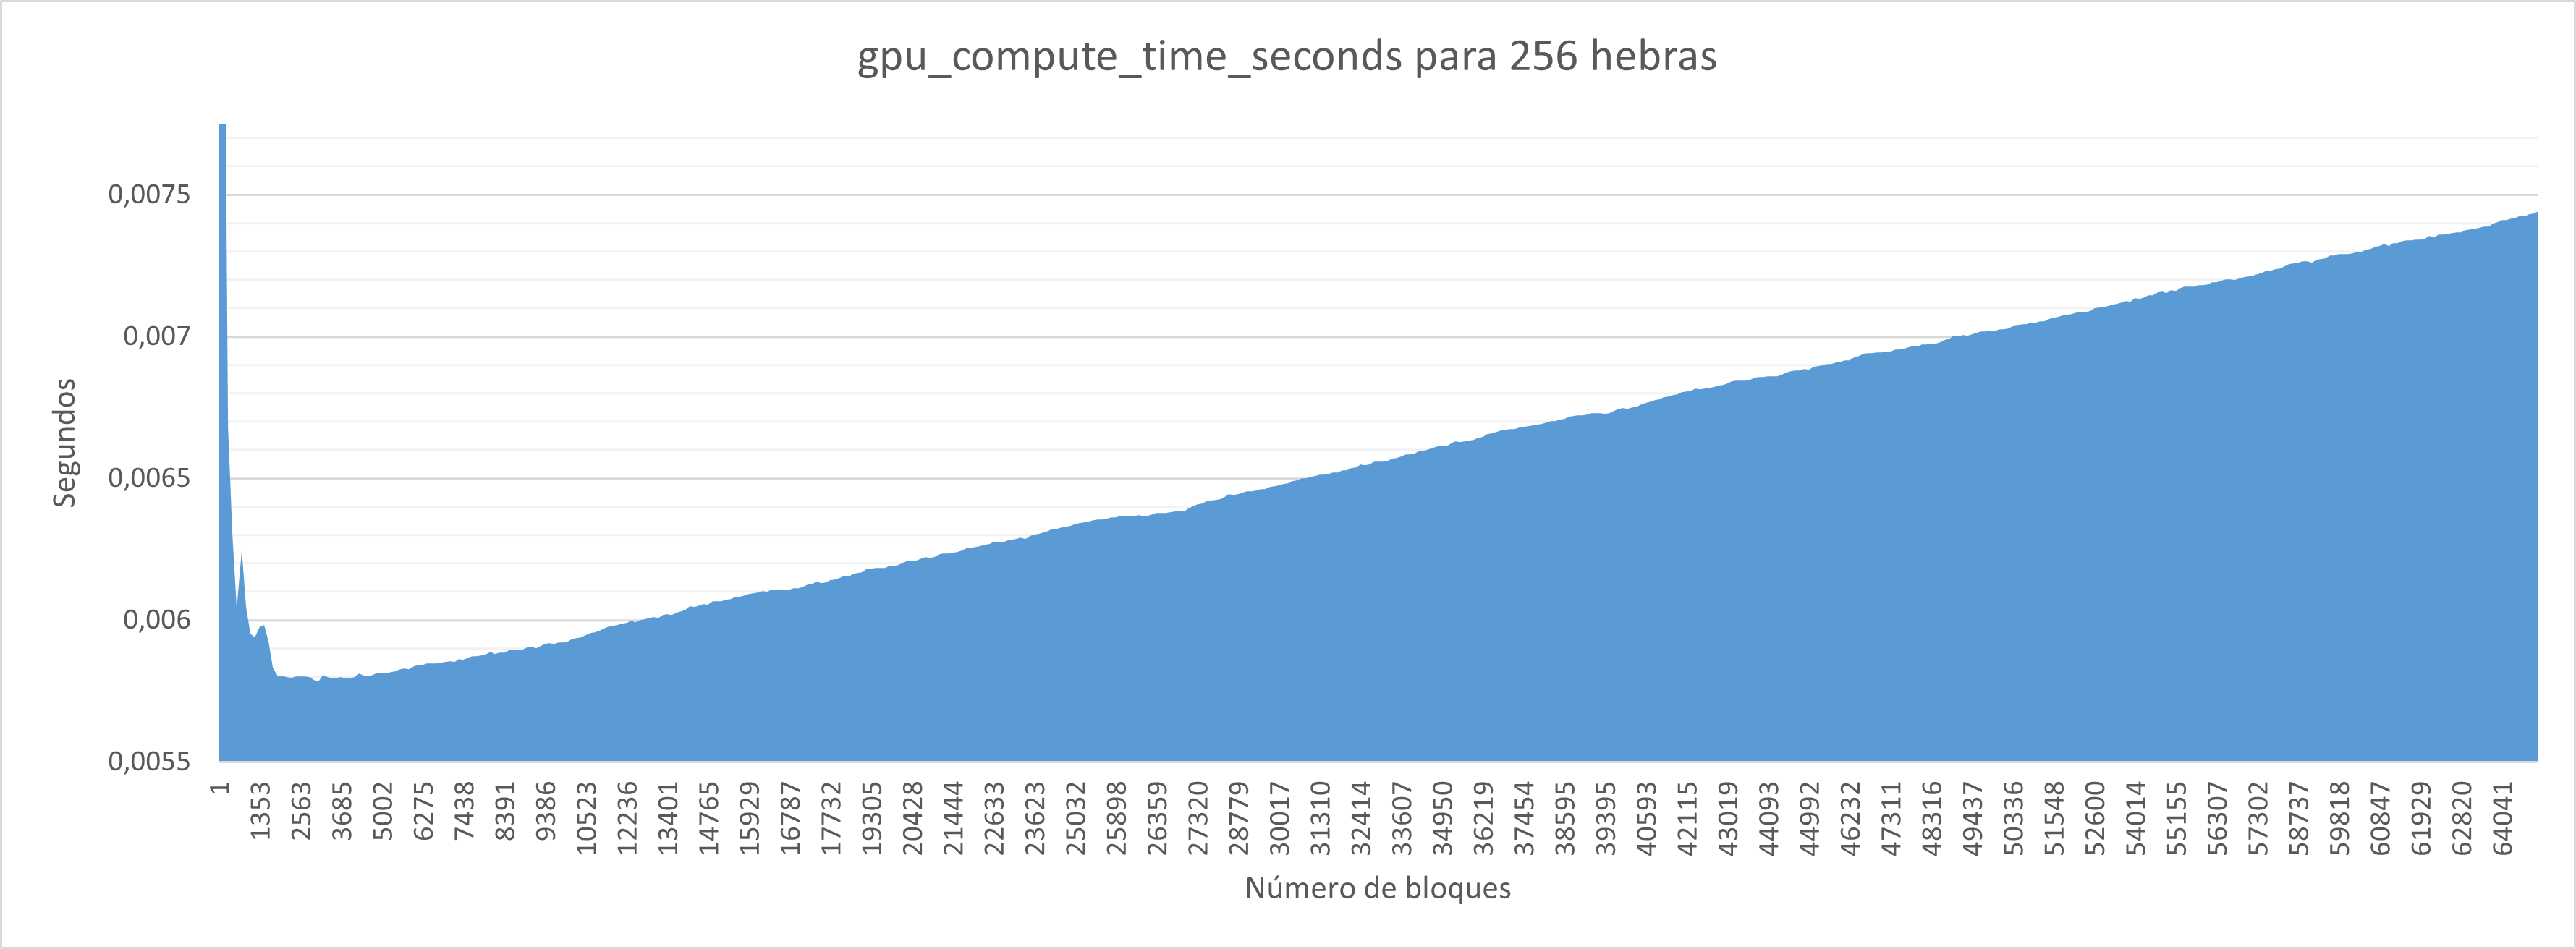
\includegraphics[width=16.75cm]{experimento_1.png}
    \caption{Tiempo medio de ejecución en GPU según el número de bloques sin contar transferencias.
    Destacan tanto el overhead síntoma de lanzar a planificar bloques con cargas nimias o inexistentes
    como la penalización resultante de lanzar a ejecutar bloques con grandes cargas.}
\end{figure}

Para evitar posibles sesgos por utilizar un tamaño de cuadrícula múltiplo de algún número vamos incrementando
aleatoriamente dentro de una cota el tamaño de cuadrícula, de forma que después de ejecutar el experimento
podamos obtener un gráfico más o menos fiel a la realidad.

Sospechamos que existe correlación entre el tamaño
de datos de entrada para el algoritmo y el número de bloques que lanzamos a ejecutar.

\section{Segundo experimento.}

Una vez obtenemos los resultados del primer experimento lanzamos el segundo experimento. Al
igual que en el experimento anterior, utilizamos incrementos aleatorios.

\begin{figure}[H]
    \centering
    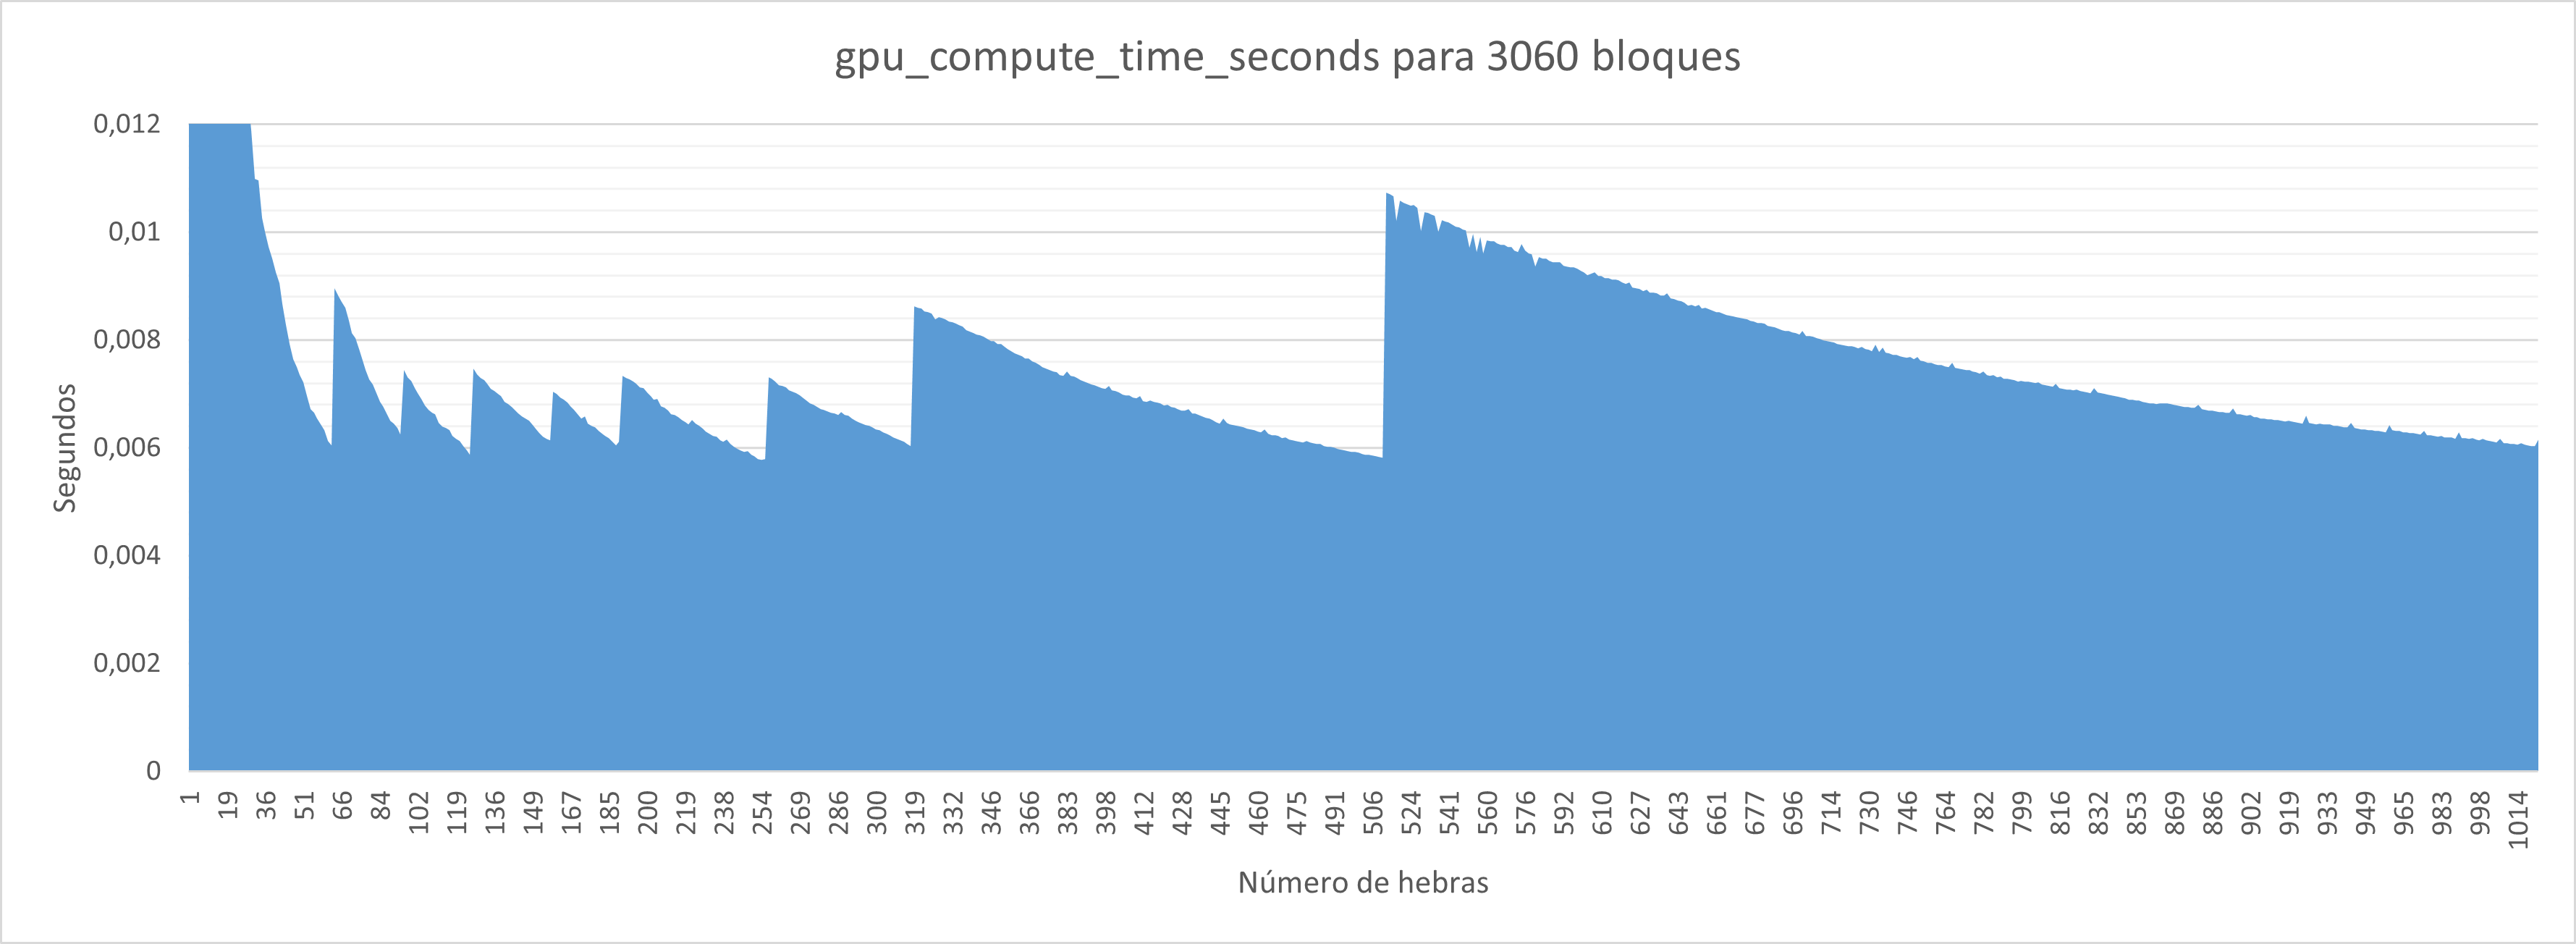
\includegraphics[width=\textwidth]{experimento_2.png}
    \caption{Tiempo medio de ejecución en GPU según el número de hebras sin contar transferencias.
    Lo primero que observamos es el patrón que se repite según se va aumentando el número de hebras lanzadas,
    los primeros con múltiplos de 32 hebras, y los siguientes con múltiplos de 64, 96 y 512. Seguidamente
    apreciamos cómo para un número de hebras inferior a 128 el rendimiento es significativamente inferior, así
    como para un número de hebras a 512.}
\end{figure}

En este experimento, a diferencia del anterior, el nivel de ocupación de la GPU está condicionada por el número
de hebras que lanzamos al invocar el \textit{kernel}, independientemente de la carga de datos. Esto es causa del
funcionamiento de la arquitectura CUDA.

De una forma simplificada y poco rigurosa, para poder ejecutar un bloque
necesitamos esperar a que tengamos un \textit{streaming multiprocessor} el cual disponga de suficientes
\textit{warps} libres donde lanzar y intercalar la ejecución de paquetes de 32 hebras. El número de hebras
que lancemos influirá en las decisiones de los distintos planificadores, que junto a otros factores como pueden ser el compilador
o los fallos de caché en tiempo de ejecución, determinará el nivel de ocupación de las estaciones de servicio de la
GPU.

\section{Tercer experimento.}

Por último, para los mejores casos de los experimentos anteriores, calculamos el \textit{speedup} con respecto al algoritmo
que podemos ejecutar en la CPU.

\begin{table}[H]
    \centering
    \begin{tabular}{|c|c|}
    \hline
    \textbf{Aceleración GPU} & \textbf{Aceleración GPU incluyendo transferencias de memoria} \\ \hline
    48,00664819     & 11,00000401                    \\ \hline
    \end{tabular}
    \caption{Aceleración obtenida para el caso en que utilizamos 3060 bloques y 256 hebras sobre el algoritmo
    que se ejecuta sobre CPU en una sola hebra.}
\end{table}

\section{Trabajo futuro.}

Para comprender mejor qué ocurre \textit{detrás del telón} a la hora de ejecutar nuestro algoritmo podríamos
someterlo a herramientas de \textit{profiling}, como puede ser \textit{NVIDIA NSight}. Esta herramienta también
nos puede proporcionar otro tipo de información como son los tamaños de cuadrilla y bloque para conseguir
una buena ocupación. También podríamos investigar otras opciones de acceso a memoria desde la GPU, si las hubiese,
u otras formas de optimizar en caso de que fuese necesario.
